
\documentclass{beamer}

\mode<presentation>
{
  \usetheme{Warsaw}
  \setbeamercovered{transparent}
}
\usepackage[english]{babel}
\usepackage[latin1]{inputenc}
\usepackage{times}
\usepackage[T1]{fontenc}

\usepackage{graphicx}
\usepackage{capt-of}
\usepackage{booktabs}
\usepackage{varwidth}

\newcommand{\N}{\mathbb{N}}
\newcommand\Fontvi{\fontsize{8}{8.2}\selectfont}

% Or whatever. Note that the encoding and the font should match. If T1
% does not look nice, try deleting the line with the fontenc.


\title[Dynamic connexity $\&$ parameterised complexity]
{Dynamic connexity $\&$ parameterised complexity}

\subtitle
{Kernelization algorithms: from static to dynamic graphs}

\author[Meyer]
{Pierre~Meyer}

\institute[Universities of Somewhere and Elsewhere]
{
  Department of Computer Science\\
  Ecole Normale Superieure de Lyon}

\date[SL3 2017]
{Soutenance de stage de fin de licence, 2017}

\subject{Theoretical Computer Science}

\pgfdeclareimage[height=0.5cm]{logoENS}{logoENS}
\logo{\pgfuseimage{logoENS}}

% Delete this, if you do not want the table of contents to pop up at
% the beginning of each subsection:
\AtBeginSubsection[]
{
  \begin{frame}<beamer>{Outline}
    \tableofcontents[currentsection,currentsubsection]
  \end{frame}
}

\expandafter\def\expandafter\insertshorttitle\expandafter{%
  \insertshorttitle\hfill%
  \insertframenumber\,/\,\inserttotalframenumber}

\begin{document}

\begin{frame}
  \titlepage
\end{frame}

\begin{frame}{Outline}
  \tableofcontents
  % You might wish to add the option [pausesections]
\end{frame}

\section{Initial problem: Sparse-split link stream editing}

\subsection{Link streams and edition}
\begin{frame}{Link streams}
  \begin{block}{Definition}
    A \emph{\bfseries link stream} is a triple $L=(T,V,E)$ where:
    \begin{itemize}
    \item $T=[0,t_{max}]$ : time interval
    \item $V$ : finite set of nodes
    \item $E$ : set of \emph{\bfseries links} ($b$, $e$, $uv$) ($b,e\in T,\ u,v\in V$)
    \end{itemize}
  \end{block}
  \begin{table}[!h]
    \begin{minipage}{0.4\linewidth}
      \centering
      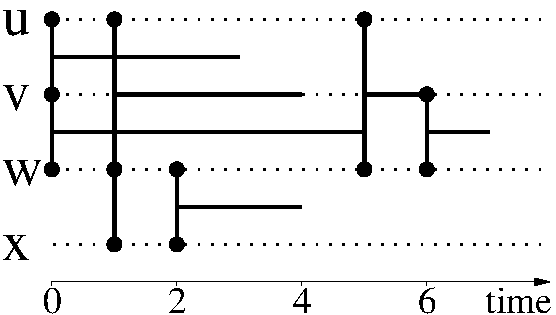
\includegraphics[width=45mm]{exviard.pdf}
      \label{fig:exviard}
    \end{minipage}
    \begin{minipage}{0.4\linewidth}
      \centering
      \begin{tabular}{c c}
        \toprule
        Pair & $(b,e)$\\
        \midrule
        $uv$ & (0,3) \\
        $uw$ & (1,4) (5,6) \\
        $vw$ & (0,2) (6,7) \\
        $ux$ & (1,5) \\
        $wx$ & (2,4) \\
        \bottomrule
      \end{tabular}
    \end{minipage}
  \end{table}
\end{frame}
\begin{frame}{Link streams - Edition}
  Link edition operation: adding/deleting a portion of link (except splitting a link in two)
  \Fontvi
  \begin{table}[!h]
    \begin{minipage}{0.3\linewidth}
      \centering
      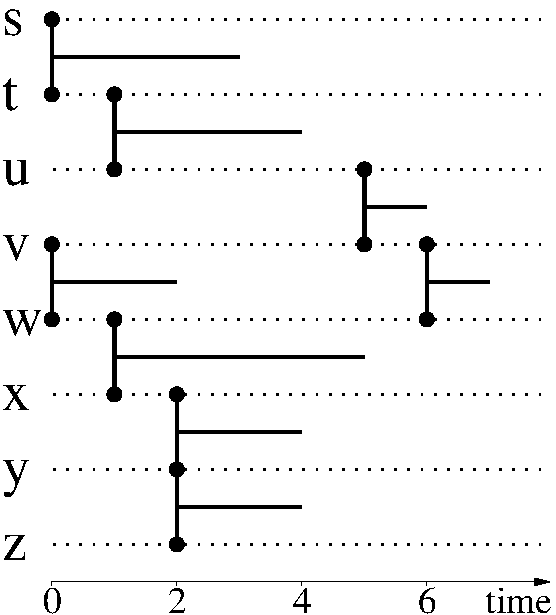
\includegraphics[width=30mm]{ex_op0.pdf}
    \end{minipage}
    \begin{tabular}{c c c c}
      \toprule
      Edge & Op type & $b$ & $e$\\
      \midrule
      $st$ & Add & 4 & 6 \\
      $tu$ & Add & 4 & 5 \\
      $uv$ & Add & 3 & 5 \\
      $vw$ & Add & 2 & 6 \\
      $wx$ & Del & 1 & 5 \\
      $xy$ & Del & 3 & 4 \\
      $yz$ & Del & 2 & 3 \\
      \bottomrule
    \end{tabular}
    \begin{minipage}{0.3\linewidth}
      \centering
      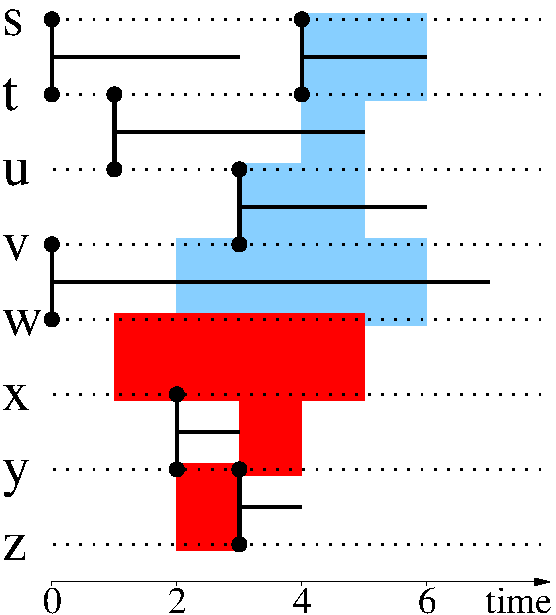
\includegraphics[width=30mm]{ex_op1.pdf}
    \end{minipage}
  \end{table}
  %In other words, all edition operations have a cost of one, no matter the length of the link to be added or deleted, and the only operation we do not allow is deleting a sub-link in the middle of a link.
\end{frame}

\subsection{Sparse-split link stream editing problem}
\begin{frame}{Sparse-split link stream} 
  \begin{block}{Sparse-Split}
    A link stream is sparse-split iff:
    \begin{itemize}
    \item All links have the same timestamps $(b_c,e_c,\_ )$
    \item It consists of ``a clique plus isolated vertices''
    \end{itemize}
  \end{block}
  \begin{minipage}{1\linewidth}
    \centering
    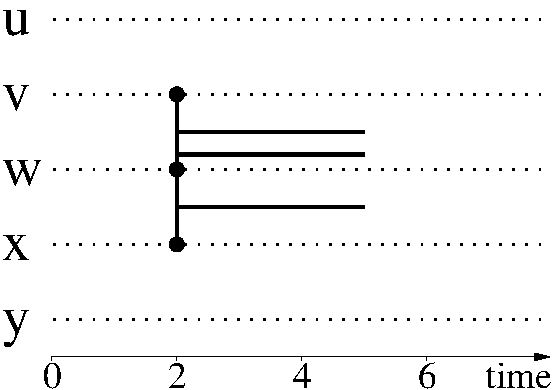
\includegraphics[width=40mm]{sparse-split.pdf}
  \end{minipage}
\end{frame}
\begin{frame}{The Sparse-Split Link Stream Editing problem (\emph{\bfseries SS-Dyn})}
  \begin{block}{Definition}
    \begin{itemize}
    \item \emph{\bfseries Input:} A link stream $L$ and an integer $k$
    \item \emph{\bfseries Output:} A list of at most $k$ edition operations which transform $L$ into a sparse-split link stream
    \end{itemize}
  \end{block}
  \begin{block}{Theorem}
    \emph{\bfseries SS-Dyn(k)} is NP-complete
  \end{block}
\end{frame}

\subsection{Parameterised complexity}
\begin{frame}
  \begin{block}{Fixed Parameter Tractability (FPT)}
    A parameterised problem is \emph{\bfseries fixed parameter tractable} is it can be solved in time $O(f(k).poly(|x|+k))$
  \end{block}
  \begin{block}{Kernelization algorithm}
    \begin{itemize}
    \item \emph{\bfseries Input:} An instance ($I$, $k$)
    \item \emph{\bfseries Output:} An equivalent instance ($I'$, $k'$) such that:
      \begin{itemize}
      \item $|I'|\leq f(k)$ for some computable function $f\ :\ \N\rightarrow \N$
      \item $k'\leq k$
      \end{itemize}
    \item \emph{\bfseries Runtime:} Polynomial in $(|I|+k)$
    \end{itemize}
  \end{block}
\end{frame}

\section{Kernelization algorithm for SS-Dyn}
\begin{frame}{Kernelization Algorithm - Overview}
  \begin{minipage}{1\linewidth}
    \centering
    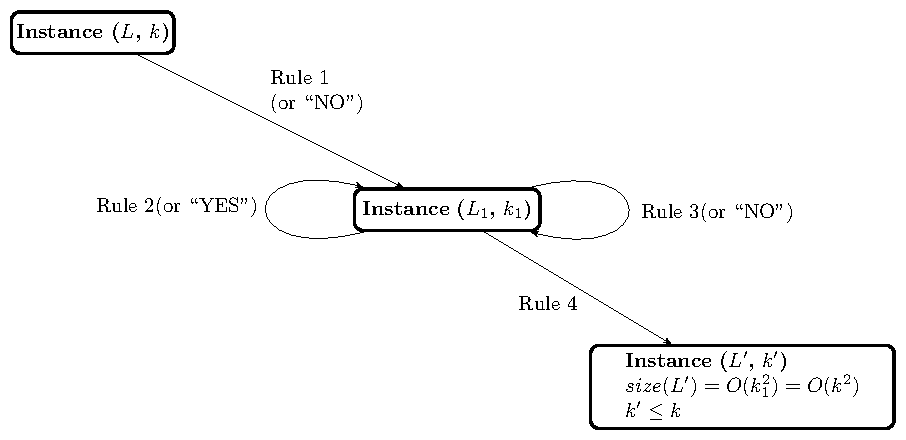
\includegraphics[width=110mm]{chart.pdf}
  \end{minipage}  
\end{frame}
\subsection{Rule Graph}
\begin{frame}
  \begin{block}{Rule 1: Rule Graph}
    \begin{itemize}
    \item \emph{\bfseries Step 1:} Remove any link which does not start at $b_c$ and/or end at $e_c$
    \item \emph{\bfseries Step 2:} If there remain two links between $u$ and $v$, merge them together
    \end{itemize}
  \end{block}
  \begin{table}[!h]
    \begin{minipage}{0.3\linewidth}
      \centering
      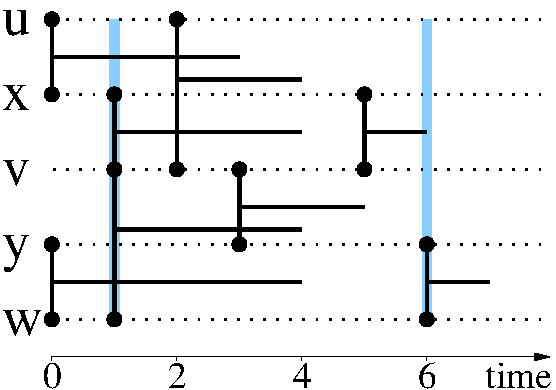
\includegraphics[width=30mm]{ex_closest0.pdf}
      \captionof{figure}{Before}
    \end{minipage}
    \begin{minipage}{0.3\linewidth}
      \centering
      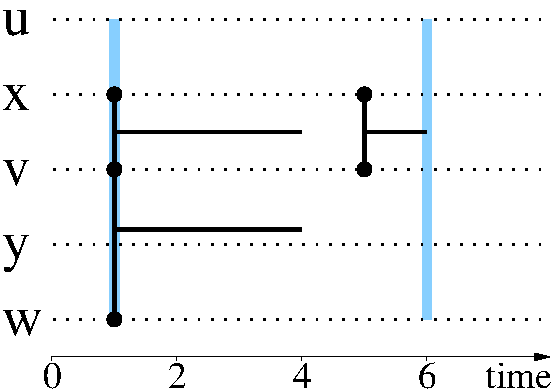
\includegraphics[width=30mm]{ex_closest01.pdf}
      \captionof{figure}{Input}
    \end{minipage}
    \begin{minipage}{0.3\linewidth}
      \centering
      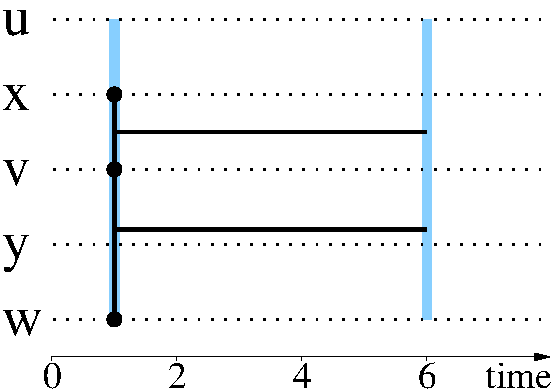
\includegraphics[width=30mm]{ex_closest1.pdf}
      \captionof{figure}{After step 2}
    \end{minipage}
  \end{table}
\end{frame}
\subsection{Rule Neighbourhood}
\begin{frame}{Rule Neighbourhood}
  \begin{block}{Rule 2: Rule Neighbourhood - Part 1}
    Consider a constant $c$~. For each vertex $u\in V_L$, try all ways of performing up to $c-1$ edition operations involving $u$, and attempt neighbourhood reconstruction.
  \end{block}
  \begin{block}{Rule 3: Rule Neighbourhood - Part 2}
    If there are more than $\frac{2}{c}k_1$ vertices with more than $c$ neighbours, then return a trivial ``no''-instance.
  \end{block}
\end{frame}
\subsection{Rule Reduce}
\begin{frame}{Rule Reduce}
  \begin{block}{Rule 4: Rule Reduce}
    Isolate any vertex with at most $c$ neighbours
  \end{block}
  \begin{block}{}
    \begin{itemize}
    \item \emph{\bfseries Runtime:} This can be done in linear time
    \item \emph{\bfseries Output:} A link stream with at most $n':=\frac{2}{c}k_1=O(k)$ vertices and $\frac{n'.(n'-1)}{2}=O(k^2)$ links
    \end{itemize}
  \end{block}
\end{frame}

\section{Generalising our results}
\subsection{Analysis: Interesting link-stream properties}
\begin{frame}{Graph-Likeness - Time intervals}
  \begin{table}[!h]
    \begin{minipage}{0.4\linewidth}
      \centering
      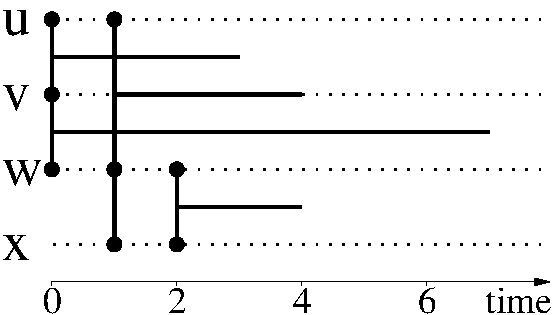
\includegraphics[width=40mm]{exintervals1.pdf}
    \end{minipage}
    \begin{minipage}{0.4\linewidth}
      \centering
      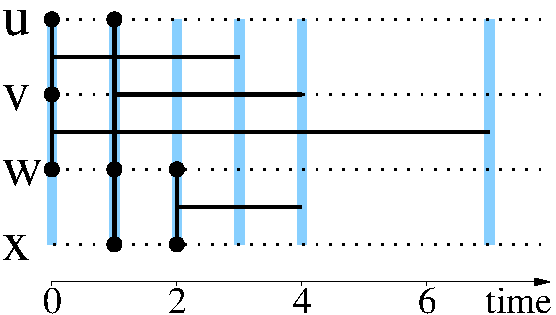
\includegraphics[width=40mm]{exintervals.pdf}
    \end{minipage}
  \end{table}
\end{frame}
\begin{frame}{Neighbourhood Reconstructibility}
  \begin{block}{definition}
    A graph-like class $\Pi$ of link streams is said to be \emph{\bfseries neighbourhood reconstructible} if there are two constants $c,d$ and an algorithm $A$ such that:
    \begin{itemize}
    \item $A$ takes as input a link stream $L$, an integer $k$, and a subset of $V_L$, $V'$, of size not greater than $d$~;
    \item $A$ runs in polynomial time in $size(L)$~;
    \item $A$ decides whether or not $L$ can be transformed, using a total of at most $k$ edition operations and less than $c$ edition operations in the vicinity of any vertex in $V'$, into a link stream $L'\in \Pi$ such that all links of $L'$ have exactly one end in $V'$~.
    \end{itemize}
  \end{block}
\end{frame}
\begin{frame}{Heredity}
  \begin{block}{Definition}
    A class of link streams is said to be \emph{\bfseries hereditary} if it is closed under vertex deletion.
  \end{block}
\end{frame}
\subsection{Synthesis: Similar problems}
\begin{frame}{Problem Denomination: First prefix}
  First prefix: Describes the maximum number of cliques of size $\geq 2$ allowed.
  \begin{itemize}
  \item \emph{\bfseries d-}
  \item \emph{\bfseries *-} (any)
  \end{itemize}
\end{frame}
\begin{frame}{Problem Denomination: Second prefix}
  Second prefix: Describes the maximum number of time intervals.
  \begin{itemize}
  \item \emph{\bfseries If there is no second prefix: } A single time interval, ie: $$\exists b_c, e_c,\ \forall l\in E_L,\ l=(b_c,e_c,\_)$$
  \item \emph{\bfseries -BI-} Two neighbouring intervals, ie: $$\exists (t_{c,i})_{i\in [0,2]},\ \forall l\in E_L,\ \exists i<j,\ l=(t_{c,i},t_{c,j},\_)$$
  \item \emph{\bfseries -MULTI-} Any number of neighbouring intervals $$\exists k,\ \exists (t_{c,i})_{i\in [0,k]},\ \forall l\in E_L,\ \exists i<j,\ l=(t_{c,i},t_{c,j},\_)$$
  \end{itemize}
\end{frame}
\begin{frame}{Problem Denomination: Stem}
  Stem: Describes whether or not we count isolated vertices when counting cliques.
  \begin{itemize}
  \item \emph{\bfseries -Sparse-Split} On each interval, the link stream is a certain number of cliques plus isolated vertices
  \item \emph{\bfseries -Cluster} On each interval, the link stream is a set of disjoint cliques
  \end{itemize}
\end{frame}
\begin{frame}{Problem Classification}
  \begin{minipage}{1\linewidth}
    \centering
    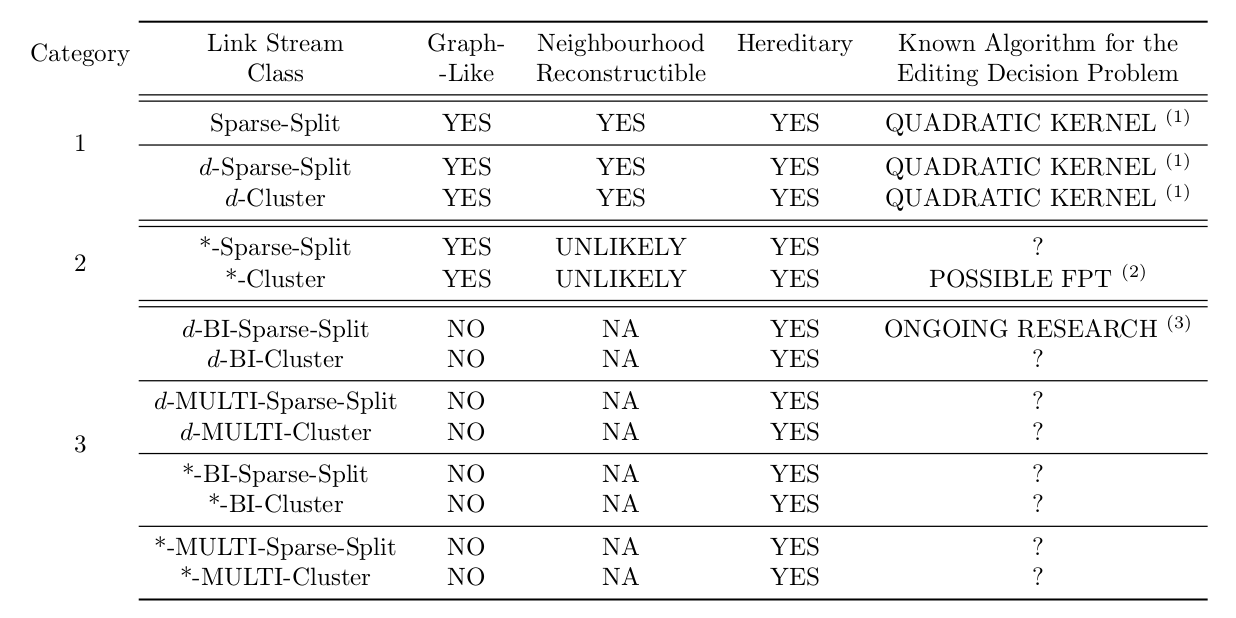
\includegraphics[width=110mm]{perspectives.png}
  \end{minipage}
\end{frame}

\section*{Summary}

\begin{frame}{Summary}
  \begin{itemize}
  \item
    The Sparse-Split Link Stream Editing problem is FPT
  \item
    Many variations thereupon are also FPT
  \end{itemize}
\end{frame}

\end{document}
